\documentclass[12pt,notitlepage]{article}

%\usepackage[LY1]{em}
%\usepackage{a4wide}
\usepackage{fancyhdr}
%\usepackage{BTkit}
%\usepackage{Bdefs}
%\usepackage{url}
\usepackage[dvipsnames]{xcolor}
\usepackage{graphicx}

% Additional packages not from template
\usepackage[hyphens]{url}
\usepackage[hmargin=0.75in, vmargin=1.25in]{geometry}
\usepackage[british]{babel}
\usepackage[backend=biber, style=apa]{biblatex}
\usepackage{hyperref}
\usepackage{xpatch}
\usepackage{multicol}
\usepackage{csquotes}
\usepackage{amsmath}
\usepackage{pdfpages}
\usepackage{float}
\usepackage{appendix}
\usepackage{enumitem}
\usepackage{booktabs}
\usepackage{tabularx}
\usepackage{multirow}

% Manage bibliography with Biblatex instead of Bibtex
\DeclareLanguageMapping{british}{british-apa}
\addbibresource{reference.bib}
\renewcommand*{\multicitedelim}{\addsemicolon\space}
\xapptobibmacro{finentry}{\par\printfield{annotation}}{}{}

% Define single column figures
\newenvironment{Figure}
  {\par\medskip\noindent\minipage{\linewidth}}
  {\endminipage\par\medskip}

\title{Dynamic Bayesian Networks for Decision Support: \\UK Vegetable Supply Model\\\& GUI for Model Outputs}
\author{Lee Sheng Long (23318325)\\
\href{mailto:sllee26@student.monash.edu}{sllee26}@student.monash.edu\\
\href{mailto:s.lee.21@warwick.ac.uk}{s.lee.21}@warwick.ac.uk\\
\url{https://github.com/slee21}
}

\lhead{Monash University Research Projects Abroad 2017}
\chead{}
\rhead{Lee Sheng Long (23318325)}
\headheight=16pt

\begin{document}
\newgeometry{hmargin=1.0in, vmargin=0.75in}
% Title page
\date{19th March 2017}
\maketitle

\begin{multicols}{2}
\tableofcontents
\end{multicols}

%Essay content
\clearpage
\restoregeometry
\setcounter{page}{1}
\pagenumbering{arabic}
\pagestyle{fancy}
\begin{multicols}{2}
\section{Introduction}\label{sec:introduction}
I spent 8 weeks in January and February of 2017 doing research projects under supervision by Dr. Martine J. Barons, Professor Ann E. Nicholson and Professor Jim Q. Smith.

The first project was to model UK vegetable supply with Bayesian Networks. It was more research-based.

The second project was to develop a simple Graphical User Interface (GUI) for model outputs. It was more application-based.
\section{UK Vegetable Supply Model}\label{sec:statsmodel}
\subsection{Motivation}
The recent UK vegetable shortage illustrated the utility and importance of the project \parencite{bbc2017}. 

Such a model could be useful to discover key factors behind the shortage and guide corrective measures to alleviate the shortage and prevent further recurrences. It could also predict price movements allowing time to prepare.

The resultant UK vegetable supply network would be integrated into a larger network based on the CPI food basket to model overall food supply in the UK.

It would ultimately contribute to a Decision Support System (DSS) for policy makers in the area of food security.
\subsection{Results}
The resultant partially parametrised Bayesian Network is described in \ref{subsubsec:network1} and is available for download at \url{https://github.com/slee21/murpa}.
\subsection{Limitations}
Time constraints resulted in some limitations:
\begin{itemize}
\item Network is only partially parametrised with Conditional Probability Tables (CPT)
\item Expert elicitations only involved 1 expert, Rob Lillywhite of Warwick Crop Centre
\end{itemize}
\subsection{Future Work}
Potential productive avenues for future work:
\begin{itemize}
\item Fully parametrize the network with CPTs
\item Expert elicitations with more experts
\item Sensitivity analysis on the network
\end{itemize}
\section{GUI for Model Outputs}\label{sec:guidevel}
\subsection{Motivation}
The Netica software package interface is targeted at practitioners familiar with Bayesian Networks, statistics and probability. 

Most policy makers likely lack the requisite knowledge and would be confused operating the Netica interface. Thus, a new interface targeted at policy makers would be useful.

The resultant GUI would provide a user-friendly interface for display and interaction with the model outputs aimed at policy makers with little background in statistics.
\subsection{Results}
The resultant frontend GUI is described in \ref{subsubsec:network1} and is available for download at \url{https://github.com/slee21/bayeslayers}. The backend JSON API server is available for download at \url{https://github.com/slee21/gonetica}.
\subsection{Limitations}
Time constraints resulted in some limitations:
\begin{itemize}
\item Saving data to and loading data from local files remains unimplemented
\item Interface look and feel is rudimentary and unpolished
\item Hardcoded or unconfigurable options and settings
\end{itemize}
\subsection{Future Work}
Potential productive avenues for future work:
\begin{itemize}
\item Implement local file saving and loading
\item Implement server side saving and loading
\item Redesign and polish interface look and feel
\item Expand configurable options and settings
\item Implement distributed collaboration
\item Redesign and optimize transfer protocol
\end{itemize}
\section{Key Takeaways}\label{sec:takeaways}
\subsection{Insight into Academia}
I had the opportunity to speak with non-teaching academics which would otherwise be difficult as an undergraduate. I also met PhD candidates and other postgraduate students. They provided different perspectives of academia.
\subsection{Research Experience}
I learned the dreadful practicality of Bayesian Networks. They were particularly useful when data was scarce. This was readily apparent in the modeling of the UK vegetable supply where often times the only sources were human wisdom.
\subsection{Development Experience}
I experienced the difficulties of working with a closed-source proprietary API (Netica API). I also gained the experience of developing a simple JSON API server and accompanying single page web application client.
\section{Conclusion}\label{sec:conclusion}
MURPA was a valuable learning experience in many ways. It helped settle most of my doubts or worries about continuing on towards honours. 

I want to thank my supervisors Dr. Martine J. Barons, Professor Ann E. Nicholson and Professor Jim Q. Smith for their kind guidance. 

I also want to thank Dr. Arun Konagurthu and Caitlin Slattery for enabling and supporting the MURPA program.

Finally, I would like to apologise for any shortcomings on my part and wish any successor MURPA students reading this all the best with your projects.
\end{multicols}

\clearpage
\printbibliography

\clearpage
\pagenumbering{roman}
\appendix
\appendixpage
\addappheadtotoc

\begin{multicols}{2}
\section{Progress Reports}\label{sec:progress}
\subsection{Arrival Report}\label{subsec:arrival}
First week was spent settling in. Check-in to accommodation, ID collection, visa confirmation and work space allocation went smoothly. 

First meeting with supervisor Dr. Martine J. Barons determined the projects for the 8 week duration at University of Warwick:
\begin{itemize}
\item Model UK vegetable supply with Dynamic Bayesian Networks (DBN) in Netica
\item Develop Graphical User Interface (GUI) to interact with and display model outputs
\end{itemize}
Expert meetings for the projects were scheduled:
\begin{itemize}
\item 12th January 2017

Meeting with Andy Davis of Warwickshire County Council to discuss the intended users and use cases of the GUI
\item 26th January 2017

Meeting with Rob Lillywhite of Warwick Crop Centre to discuss the UK vegetable supply Bayesian Network structure
\end{itemize}

\subsection{Progress Report: 09/01/2017 to 20/01/2017}\label{subsec:progress1}
The UK vegetable supply model was put on the backburner for most of the 2 week period. It was mainly due to the timing of the expert meetings.

Prior to meeting with Andy Davis, several broad possibilities were identified for the GUI:
\begin{enumerate}[label=(\Alph*)]
\itemsep0em 
\item Bespoke native application
\item Application plug-in or extension
\item In-browser web application
\end{enumerate}

Of the three options, I most favoured \textbf{(C)} as it targets any platform with a web browser without much additional effort.

After meeting with Andy Davis, we decided to go with option \textbf{(C)} as it was the most similar to what was in use internally at the Warwickshire City Council\footnote{\url{http://www.warwickshire.gov.uk/gis}}. Familiarity reduces barriers to software adoption.

Further, a key element of the proposed GUI would be a geographical map to visualise model outputs at various governmental scales - region, county, district and so on. The niche is well-established with giants such as Google Maps.

I tentatively decided to use the same major components as the Warwickshire City Council\footnote{\url{http://www.ordnancesurvey.co.uk/business-and-government/case-studies/warwickshire-county-council-new-web-gis.html}}. The intention was to reduce the maintenance burden as far as reasonably possible. It also helps reduce the scope of development.

However, no existing glue code between the modelling software and the GUI software stack was found. It was necessary to develop custom software using the available Netica APIs\footnote{\url{http://www.norsys.com/netica_api.html}}. Of these, only the Java and C APIs were pragmatic.

The Java and C APIs were learned and test programs written sometimes with wrappers for comparison purposes. The programs performed batch inference given input Bayesian Network and cases. Interactive versions would follow after.

Scattered time was spent reading literature on UK vegetable supply.
\end{multicols}

\begin{multicols}{2}
\subsection{Progress Report: 23/01/2017 to 03/02/2017}\label{subsec:progress2}
An initial Bayesian Network \ref{subsec:network0} was drawn up in Netica in preparation for the meeting with Rob Lillywhite.

It follows the recommendations contained in the MURPA 2016 report by Joshua Collins. The final fruit network by Sophia Wright was used as a reference because fruit was the most similar of the mapped Consumer Price Index (CPI) classes. 

After the meeting with Rob Lillywhite, it was clear that the initial model needed more precise definition and further adjustment.

First, vegetables as defined by the UK CPI basket of goods and services\footnote{\cite{ons2016a}} include a variety of crops with different properties. For example, some vegetables may be stored whereas others deteriorate quickly after harvesting.

Therefore, it may be appropriate to focus the model on a subset of exemplar vegetables that have similar properties. Also, not all vegetables may be relevant from a food security standpoint. Expensive luxury items may be excluded.

Following are comments on the structure of the initial model -- the nodes and edges of the Bayesian Network.

The production cost of vegetables does not significantly affect the vegetable production volume. The production cost is passed on to the buyer by increasing the selling price. Thus, it affects vegetable price instead of production.

Weather has a widespread impact and does not only affect vegetable production. It likely affects more variables than in the initial model. Additionally, world climate change is not the sole determinant of UK weather conditions.

Pollinators are beneficial to some vegetables but their impact on vegetables in aggregate is not significant. Similarly, organic methods yield significantly less produce but are a niche market likely irrelevant to food security.

Biofuel production has no significant impact on vegetable production. vegetables are not used for biofuel unlike cereals. Vegetables are also quite profitable and land for planting vegetables is unlikely to be repurposed for biofuels.

Vegetables are not attractive for research and development (R\&D) spending. The market is too small. Instead most research is done for arable crops as a whole. Even then, most R\&D spent tends to have impact only after 10 years or more.

Crop disease and pests are only a concern if available mitigation tools such as pesticides are limited. Government regulation may prohibit the use of certain active ingredients in pesticides. An example of this would be the ban on neonics\footnote{\cite{bbc2016}}.

Absent in the initial model is the significant waste (up to 30\%) that occurs in the supply chain between farm production and retailer supply.

Retailer or more specifically supermarket policy also has a significant impact on the supply of vegetables in the UK.

Labour cost and availability is also a concern. Agriculture is reliant on migrant labour (up to 90\%) which is determined by government policy.

I decided to use Go\footnote{\url{http://golang.org/cmd/cgo/}} to wrap the Netica C API and develop the backend for the GUI. The reasons were mostly pragmatic.

Although I can write scripts in Java and C, I am not confident I can deliver an application in the available time. I have more experience in Go and the compiled binaries are easy to maintain. Go is also a relatively simple language.
\end{multicols}

\begin{multicols*}{2}
\subsection{Progress Report: 06/02/2017 to 17/02/2017}\label{subsec:progress3}
Expert meetings for the projects were scheduled:
\begin{itemize}
\item 15th February 2017

Meeting with Rob Lillywhite to discuss the revised Bayesian Network structure and parameters

\item 16th February 2017

Meeting with Andy Davis to demonstrate the GUI prototype and discuss issues that arose during development of the prototype
\end{itemize}

A revised Bayesian Network \ref{subsubsec:network1} was drawn up after the first meeting with Rob Lillywhite. It attempts to incorporate the points discussed during the meeting. The nodes and states were specified in more detail in a table \ref{subsubsec:define1}.

The meeting confirmed that the structure of the revised network was reasonable. Rob also suggested more appropriate information sources for some of the nodes. Finally, he specified the Conditional Probability Table (CPT) for the ``UK Vegetable Price'' node \ref{subsubsec:cptables1}.

It was clarified that DEFRA horticulture production statistics \footnote{\cite{defra2016a}} only account for ``UK marketed produce'' which excludes supply chain waste. Thus, the ``UK Vegetable Production'' node required a different information source that included farm waste in its statistics.

DEFRA agriculture statistics \footnote{\cite{defra2016b}} only provide total production cost figures. It was suggested that vegetable specific production costs could be estimated based on cost per yield figures from literature. The ``John Nix Farm Management Pocketbook''\footnote{\cite{nix2015}} was suggested as a source.

Kantar\footnote{http://www.kantar.com/} was suggested as an authoritative information source for ``UK Vegetable Demand'' and ``UK Retailer Policy'' nodes.

Fresh Produce Journal \footnote{http://www.fruitnet.com/fpj} was suggested as an information source for ``UK Vegetable Price'' and ``World Vegetable Price'' nodes.

The CPTs for the network were elicited. However, time constraints resulted in only the partial CPT for the central ``UK Vegetable Price'' node. The remaining entries in the CPT may be interpolated\footnote{\cite{cain2001}} from the entries available in the partial CPT.

Prior to second the meeting with Andy Davis, a rough prototype GUI \ref{subsec:screens0} was developed to provide a visual frontend for the Go command line interface (CLI) backend. The GUI was a single page webapp using HTML and CSS for display and Javascript for logic.

There was a tentatively positive response to the rough prototype GUI at the meeting. Minor tweaks were suggested before a final meeting was planned for the departure week. The desired map boundaries were confirmed. Also, inference was confirmed to only produce expected values.
\subsection{Departure Report}\label{subsec:departure}
Unfortunately, progress on the GUI was blocked by some bugs. There was no significant progress to show at the final meeting.

The rest of the week was spent preparing for departure and attempting to debug the GUI Javascript frontend. Accommodation check-out went without issue. Final report was written-up.
\end{multicols*}

\clearpage
\section{Netica Networks}\label{sec:networks}
\subsection{UK Vegetable Supply BN prior to 26/01/2017 meeting}\label{subsec:network0}
\begin{center}
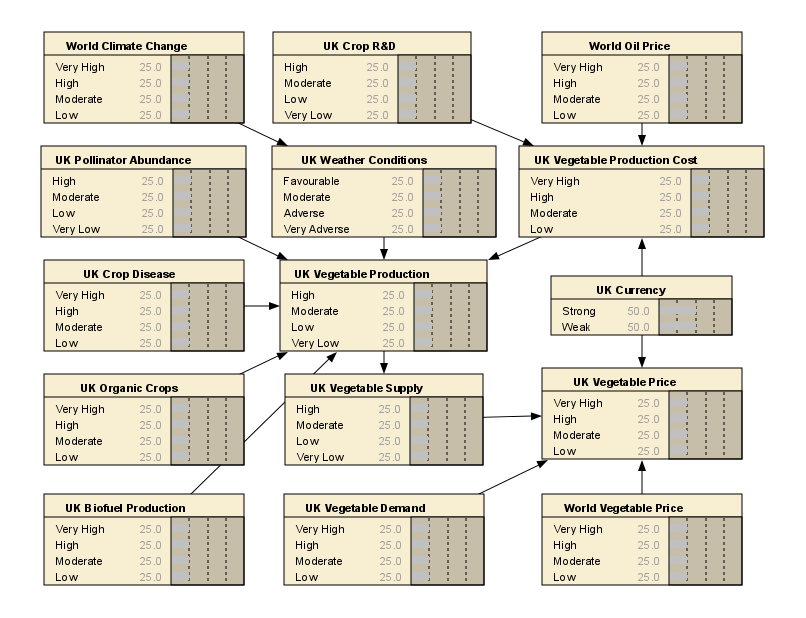
\includegraphics[width=\linewidth]{network0}
\end{center}
\subsection{Revised UK Vegetable Supply BN prior to 15/02/2017 meeting}
\subsubsection{Netica network}\label{subsubsec:network1}
\begin{center}
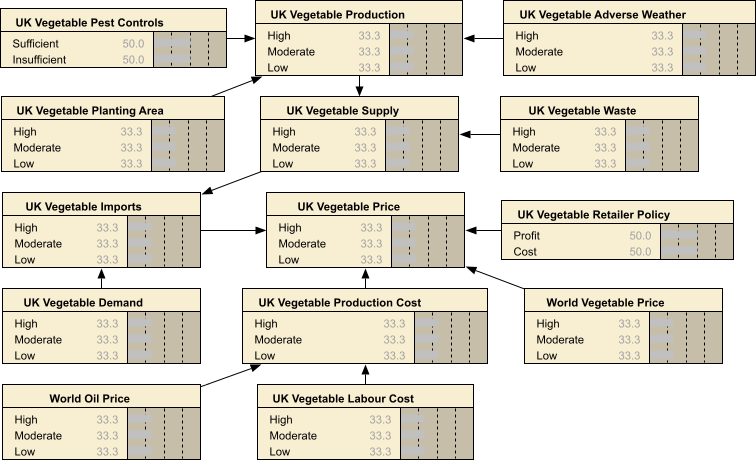
\includegraphics[width=\linewidth]{network1}
\end{center}
\subsubsection{Node and state definitions}\label{subsubsec:define1}
\begin{tabularx}{\textwidth}{
p{0.175\textwidth}p{0.275\textwidth}p{0.1\textwidth}p{0.375\textwidth}}  
\toprule
\multicolumn{2}{c}{\textbf{Node Details}}	& \multicolumn{2}{c}{\textbf{State Details}}\\
\midrule
\multirow{2}{0.175\textwidth}{\textbf{UK Vegetable Pest Controls}}
& \multirow{2}{0.275\textwidth}{Availability of pest controls such as pesticides.}
  & Sufficient 		& Any banned control has reasonable alternatives.\\
\cline{3-4}
& & Insufficient 	& Exists banned controls without any reasonable alternatives.\\
Parents & \multicolumn{3}{p{0.75\textwidth}}{None}\\
Info sources & \multicolumn{3}{p{0.75\textwidth}}{?}\\
\midrule
\multirow{2}{0.175\textwidth}{\textbf{UK Vegetable Production}}	
& \multirow{2}{0.275\textwidth}{Total production of vegetables in tonnes.}
  & High 		& \multirow{3}{0.375\textwidth}{\% change in total vegetable production relative to previous period.}\\
& & Moderate 	&\\
& & Low 		&\\
Parents & \multicolumn{3}{p{0.75\textwidth}}{UK Vegetable Pest Controls, UK Weather Conditions, UK Vegetable Planting Area}\\
Info sources & \multicolumn{3}{p{0.75\textwidth}}{\href{https://www.gov.uk/government/collections/horticultural-statistics}{Horticulture Statistics} by \href{https://www.gov.uk/government/organisations/department-for-environment-food-rural-affairs}{DEFRA}}\\
\midrule
\end{tabularx}
\begin{tabularx}{\textwidth}{
p{0.175\textwidth}p{0.275\textwidth}p{0.1\textwidth}p{0.375\textwidth}}  
\toprule
\multicolumn{2}{c}{\textbf{Node Details}}	& \multicolumn{2}{c}{\textbf{State Details}}\\
\midrule
\multirow{3}{0.175\textwidth}{\textbf{UK Vegetable Adverse Weather}}	
& \multirow{3}{0.275\textwidth}{Risk of adverse weather affecting vegetable crop such as floods.}
  & High 		& \multirow{2}{0.375\textwidth}{Average \% risk of adverse weather over the time period weighted by planting area affected.}\\
& & Moderate 	&\\
& & Low 		&\\
Parents & \multicolumn{3}{p{0.75\textwidth}}{None}\\
Info sources & \multicolumn{3}{p{0.75\textwidth}}{\href{http://www.metoffice.gov.uk/}{Met Office}}\\
\midrule
\multirow{2}{0.175\textwidth}{\textbf{UK Vegetable Planting Area}}	
& \multirow{3}{0.275\textwidth}{Total land area used for planting vegetables in hectares.}
  & High 		& \multirow{3}{0.375\textwidth}{\% change in land area used for vegetables relative to previous period.}\\
& & Moderate 	&\\
& & Low 		&\\
Parents & \multicolumn{3}{p{0.75\textwidth}}{None}\\
Info sources & \multicolumn{3}{p{0.75\textwidth}}{\href{https://www.gov.uk/government/collections/horticultural-statistics}{Horticulture Statistics} by \href{https://www.gov.uk/government/organisations/department-for-environment-food-rural-affairs}{DEFRA}}\\
\midrule
\multirow{2}{0.175\textwidth}{\textbf{UK Vegetable Supply}}	
& \multirow{2}{0.275\textwidth}{Total domestic supply of vegetables in tonnes.}
  & High 		& \multirow{3}{0.375\textwidth}{\% change in total vegetable supply less imports relative to previous period.}\\
& & Moderate 	&\\
& & Low 		&\\
Parents & \multicolumn{3}{p{0.75\textwidth}}{UK Vegetable Production, UK Vegetable Waste}\\
Info sources & \multicolumn{3}{p{0.75\textwidth}}{\href{https://www.gov.uk/government/collections/horticultural-statistics}{Horticulture Statistics} by \href{https://www.gov.uk/government/organisations/department-for-environment-food-rural-affairs}{DEFRA}}\\
\midrule
\multirow{3}{0.175\textwidth}{\textbf{UK Vegetable Waste}}	
& \multirow{4}{0.275\textwidth}{Produce lost to waste along the supply chain before reaching end consumer.}
  & High 		& \multirow{4}{0.375\textwidth}{\% proportion of vegetable waste along the supply chain before reaching end consumer over total vegetable production for the period.}\\
& & Moderate 	&\\
& & Low 		&\\
& & 			&\\
Parents & \multicolumn{3}{p{0.75\textwidth}}{None}\\
Info sources & \multicolumn{3}{p{0.75\textwidth}}{\href{http://www.wrap.org.uk/content/quantification-food-surplus-waste-and-related-materials-supply-chain}{Quantification of food surplus waste and related materials in the supply chain} by \href{http://www.wrap.org.uk/}{WRAP}}\\
\midrule
\multirow{2}{0.175\textwidth}{\textbf{UK Vegetable Imports}}
& \multirow{2}{0.275\textwidth}{Total imports of vegetables in tonnes.}
  & High 		& \multirow{2}{0.375\textwidth}{\% change in imported vegetable supply relative to previous period.}\\
& & Moderate 	&\\
& & Low 		&\\
Parents & \multicolumn{3}{p{0.75\textwidth}}{UK Vegetable Supply, UK Vegetable Demand}\\
Info sources & \multicolumn{3}{p{0.75\textwidth}}{\href{https://www.gov.uk/government/collections/horticultural-statistics}{Horticulture Statistics} by \href{https://www.gov.uk/government/organisations/department-for-environment-food-rural-affairs}{DEFRA}}\\
\midrule
\multirow{2}{0.175\textwidth}{\textbf{UK Vegetable Price}}
& \multirow{2}{0.275\textwidth}{Domestic retail price of vegetables to end consumer in \textsterling.}
  & High 		& \multirow{4}{0.375\textwidth}{\% change in Consumer Price Index (CPI) for the vegetables CPI class in the CPI basket of goods relative to previous period.}\\
& & Moderate 	&\\
& & Low 		&\\
& & 	 		&\\
Parents & \multicolumn{3}{p{0.75\textwidth}}{UK Vegetable Imports, UK Retailer Policy, UK Vegetable Production Cost, World Vegetable Price}\\
Info sources & \multicolumn{3}{p{0.75\textwidth}}{\href{https://www.ons.gov.uk/economy/inflationandpriceindices/bulletins/consumerpriceinflation/previousReleases}{UK Consumer Price Inflation} by \href{https://www.ons.gov.uk/}{ONS}}\\
\midrule
\end{tabularx}
\begin{tabularx}{\textwidth}{
p{0.175\textwidth}p{0.275\textwidth}p{0.1\textwidth}p{0.375\textwidth}}  
\toprule
\multicolumn{2}{c}{\textbf{Node Details}}	& \multicolumn{2}{c}{\textbf{State Details}}\\
\midrule
\multirow{2}{0.175\textwidth}{\textbf{UK Vegetable Retailer Policy}}
& \multirow{2}{0.275\textwidth}{Policy or treatment of vegetables as a product by retailers such as supermarkets.}
  & Profit 		& Retailer treats vegetables as products to profit from directly.\\
\cline{3-4}
& & Cost 		& Retailer treats vegetables as a cost to attract consumers so they purchase other products and profit indirectly.\\
Parents & \multicolumn{3}{p{0.75\textwidth}}{None}\\
Info sources & \multicolumn{3}{p{0.75\textwidth}}{?}\\
\midrule
\multirow{2}{0.175\textwidth}{\textbf{UK Vegetable Demand}}
& \multirow{2}{0.275\textwidth}{Total domestic demand of vegetables in tonnes.}
  & High 		& \multirow{4}{0.375\textwidth}{\% change in total vegetable supply relative to previous period. \textbf{ASSUMPTION}:\newline Total demand = Total supply}\\
& & Moderate 	&\\
& & Low 		&\\
& & 	 		&\\
Parents & \multicolumn{3}{p{0.75\textwidth}}{None}\\
Info sources & \multicolumn{3}{p{0.75\textwidth}}{?\href{https://www.gov.uk/government/collections/horticultural-statistics}{Horticulture Statistics} by \href{https://www.gov.uk/government/organisations/department-for-environment-food-rural-affairs}{DEFRA}}\\
\midrule
\multirow{3}{0.175\textwidth}{\textbf{UK Vegetable Production Cost}}
& \multirow{2}{0.275\textwidth}{Total domestic production cost of vegetables in \textsterling.}
  & High 		& \multirow{2}{0.375\textwidth}{\% change in total production cost of vegetables relative to previous period.}\\
& & Moderate 	&\\
& & Low 		&\\
Parents & \multicolumn{3}{p{0.75\textwidth}}{None}\\
Info sources & \multicolumn{3}{p{0.75\textwidth}}{?\href{https://www.gov.uk/government/collections/agriculture-in-the-united-kingdom}{Agriculture in the United Kingdom} by \href{https://www.gov.uk/government/organisations/department-for-environment-food-rural-affairs}{DEFRA}}\\
\midrule
\multirow{3}{0.175\textwidth}{\textbf{World Vegetable Price}}
& \multirow{2}{0.275\textwidth}{Global price of vegetables adjusted to \textsterling.}
  & High 		& \multirow{3}{0.375\textwidth}{\% change in world price of vegetables relative to previous period.\newline\textbf{ASSUMPTION}:\newline World price = Import price}\\
& & Moderate 	&\\
& & Low 		&\\
& & 			&\\
& &		 		&\\
Parents & \multicolumn{3}{p{0.75\textwidth}}{None}\\
Info sources & \multicolumn{3}{p{0.75\textwidth}}{?\href{https://www.gov.uk/government/collections/horticultural-statistics}{Horticulture Statistics} by \href{https://www.gov.uk/government/organisations/department-for-environment-food-rural-affairs}{DEFRA}}\\
\midrule
\multirow{2}{0.175\textwidth}{\textbf{World Oil Price}}
& \multirow{2}{0.275\textwidth}{Global price of a barrel of crude oil adjusted to \textsterling.}
  & High 		& \multirow{6}{0.375\textwidth}{\% change in average crude oil price over the period relative to previous period average.\newline\textbf{ASSUMPTION}:\newline Crude oil price is representative of world oil price.}\\
& & Moderate 	&\\
& & Low 		&\\
& & 			&\\
& &		 		&\\
& &		 		&\\
Parents & \multicolumn{3}{p{0.75\textwidth}}{None}\\
Info sources & \multicolumn{3}{p{0.75\textwidth}}{\href{http://www.nasdaq.com/markets/crude-oil.aspx}{Crude Oil Prices} at \href{http://www.nasdaq.com/}{NASDAQ}}\\
\midrule
\multirow{2}{0.175\textwidth}{\textbf{UK Vegetable Labour Cost}}
& \multirow{2}{0.275\textwidth}{Total labour cost of domestic vegetable production in \textsterling.}
  & High 		& \multirow{3}{0.375\textwidth}{\% change in total labour cost of domestic vegetable production relative to previous period.}\\
& & Moderate 	&\\
& & Low 		&\\
Parents & \multicolumn{3}{p{0.75\textwidth}}{None}\\
Info sources & \multicolumn{3}{p{0.75\textwidth}}{?\href{https://www.gov.uk/government/collections/agriculture-in-the-united-kingdom}{Agriculture in the United Kingdom} by \href{https://www.gov.uk/government/organisations/department-for-environment-food-rural-affairs}{DEFRA}}\\
\bottomrule
\end{tabularx}
\subsubsection{Conditional Probability Tables (CPTs)}\label{subsubsec:cptables1}
Transcribed below is the partial CPT for the ``UK Vegetable Price'' node elicited from Rob Lillywhite before interpolation.

\noindent\begin{tabularx}{\textwidth}{
p{0.125\textwidth}p{0.125\textwidth}p{0.125\textwidth}p{0.125\textwidth}p{0.10\textwidth}p{0.13\textwidth}p{0.10\textwidth}}  
\toprule
\multicolumn{4}{c}{\textbf{Parents}}	& \multicolumn{3}{c}{\textbf{UK Price}}\\
\cline{5-7}
\textbf{Imports} & \textbf{Retailer Policy} & \textbf{Production Cost} & \textbf{World Price} & \textbf{High} & \textbf{Moderate} & \textbf{Low}\\
\midrule
High & Profit & High & High & 90\% & 8\% & 2\%\\
High & Profit & High & Moderate & 80\% & 15\% & 5\%\\
High & Profit & High & Low & 50\% & 25\% & 25\%\\
High & Profit & Moderate & High & 90\% & 8\% & 2\%\\
High & Profit & Moderate & Moderate & 80\% & 15\% & 5\%\\
High & Profit & Moderate & Low & 70\% & 20\% & 10\%\\
Moderate & Profit & High & High & 90\% & 8\% & 2\%\\
Low & Profit & High & High & 70\% & 20\% & 10\%\\
High & Cost & High & High & 80\% & 15\% & 5\%\\
High & Cost & High & Moderate & 70\% & 20\% & 10\%\\
High & Cost & High & Low & 60\% & 30\% & 10\%\\
Low & Cost & Low & Low & 30\% & 40\% & 30\%\\
\bottomrule
\end{tabularx}
\clearpage
\section{Graphical User Interface (GUI) Screenshots}\label{sec:screens}
\subsection{GUI screenshots prior to 16/02/2017 meeting}\label{subsec:screens0}
The user may select from the list of available Bayesian Networks.
\begin{center}
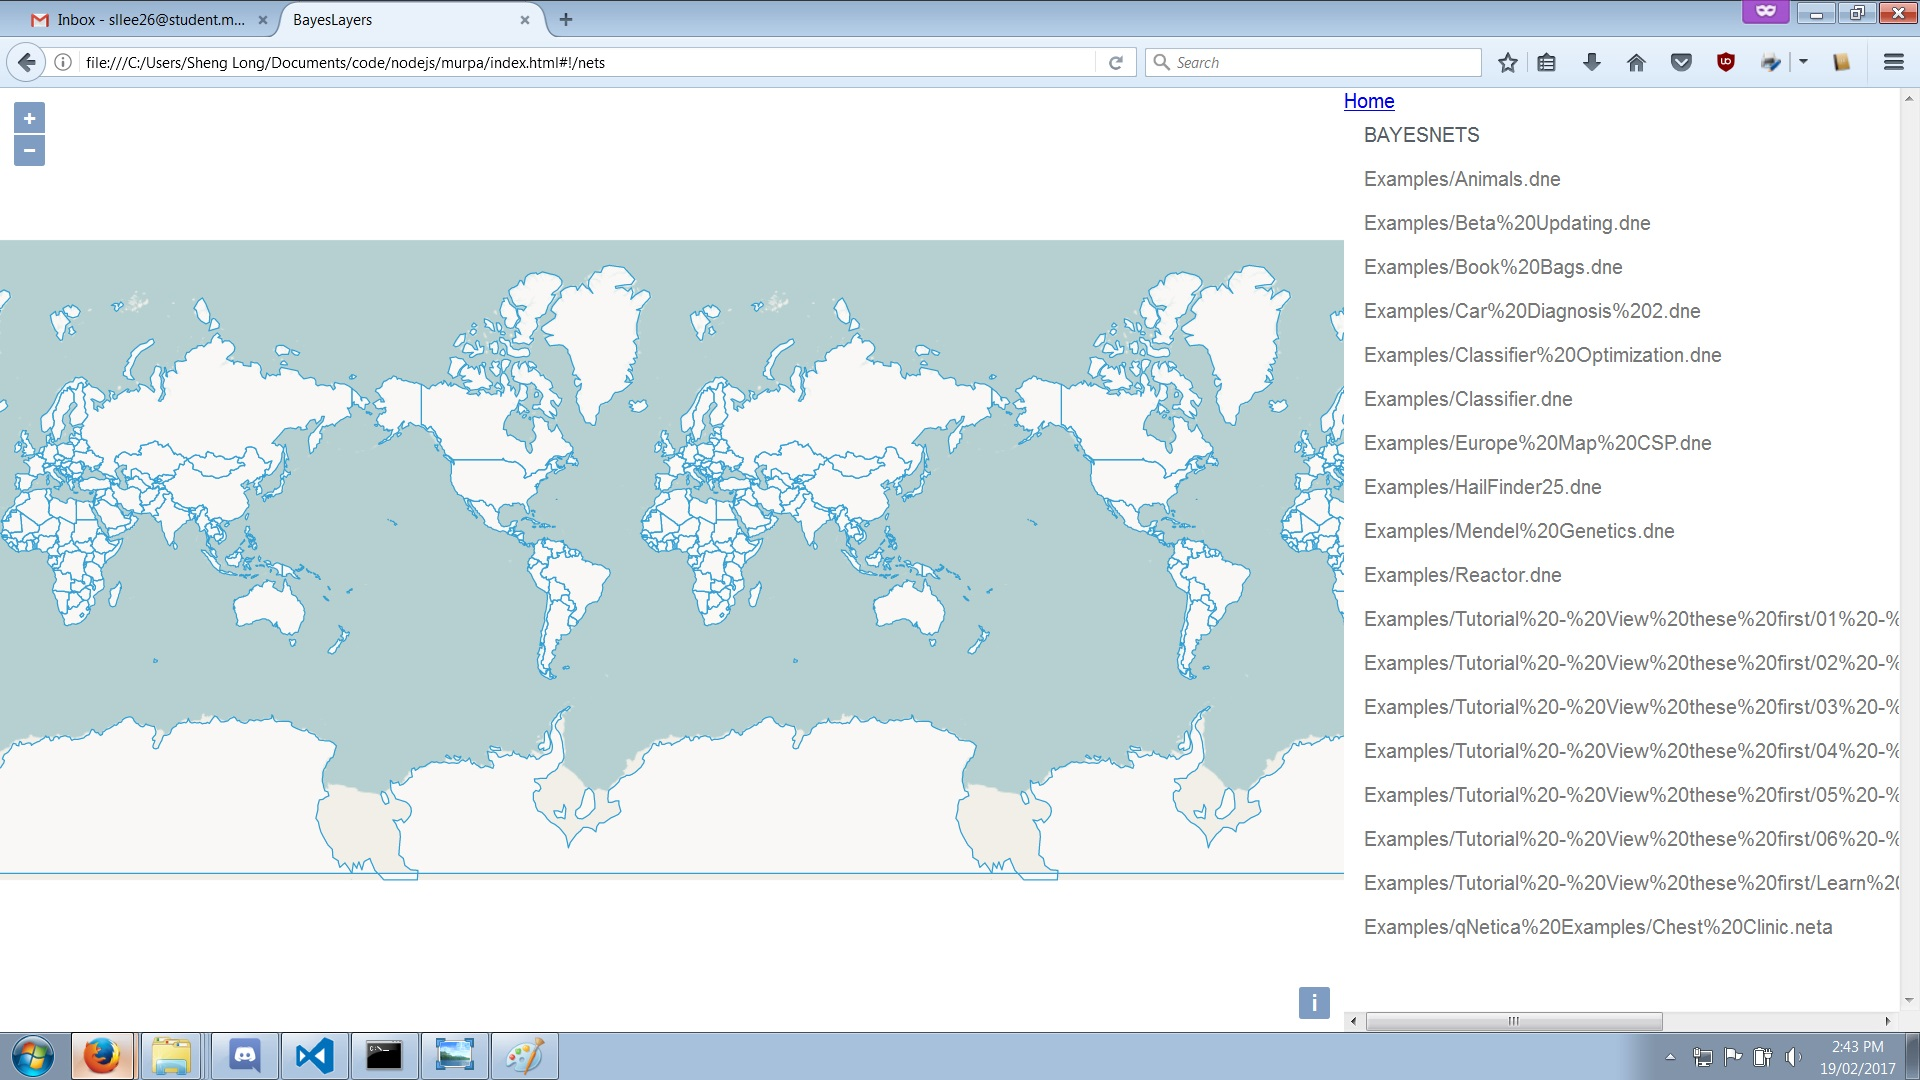
\includegraphics[width=0.8\linewidth]{v0nets}
\end{center}
Once a Bayesian Network is selected, the user may modify the node states or values associated with regions on the map.
\begin{center}
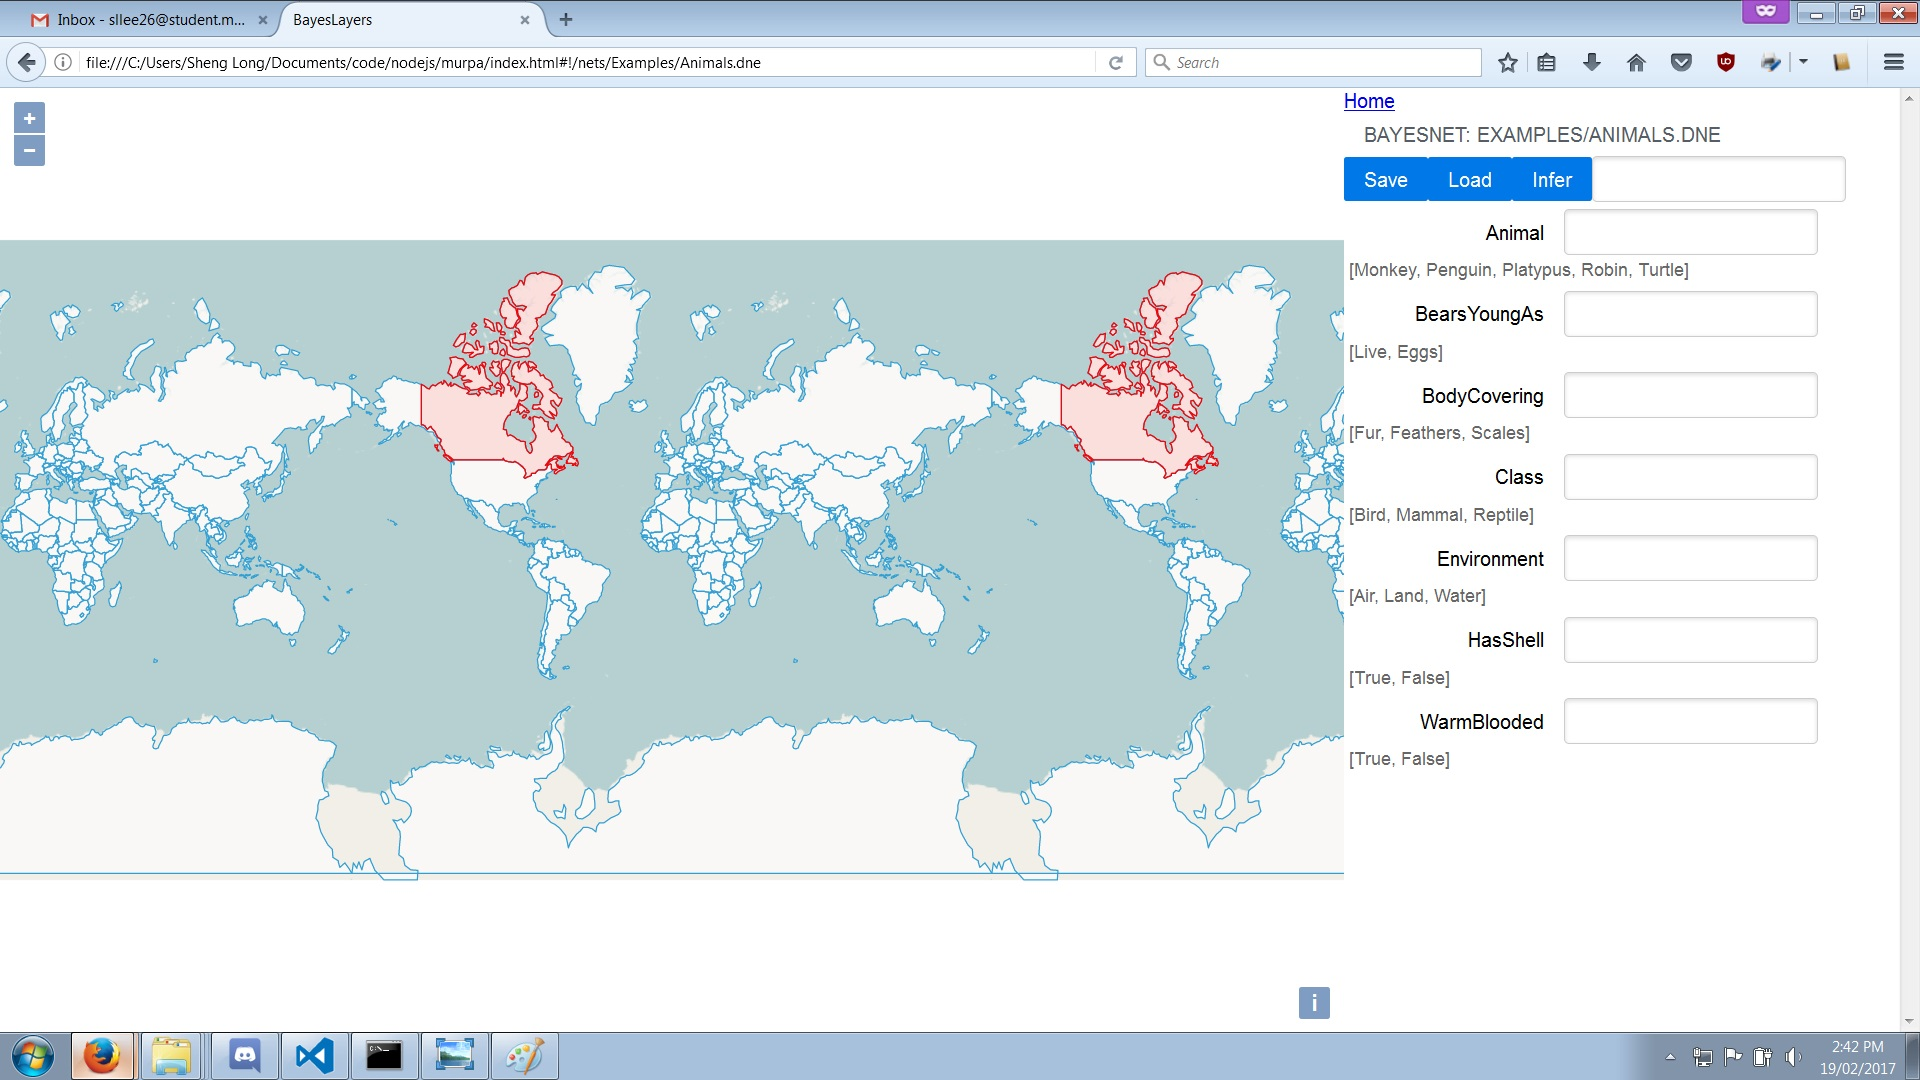
\includegraphics[width=0.8\linewidth]{v0nodes}
\end{center}
\clearpage
\noindent The user may then get the result of Bayesian inference of a desired node for the map region with entered node states and values.
\begin{center}
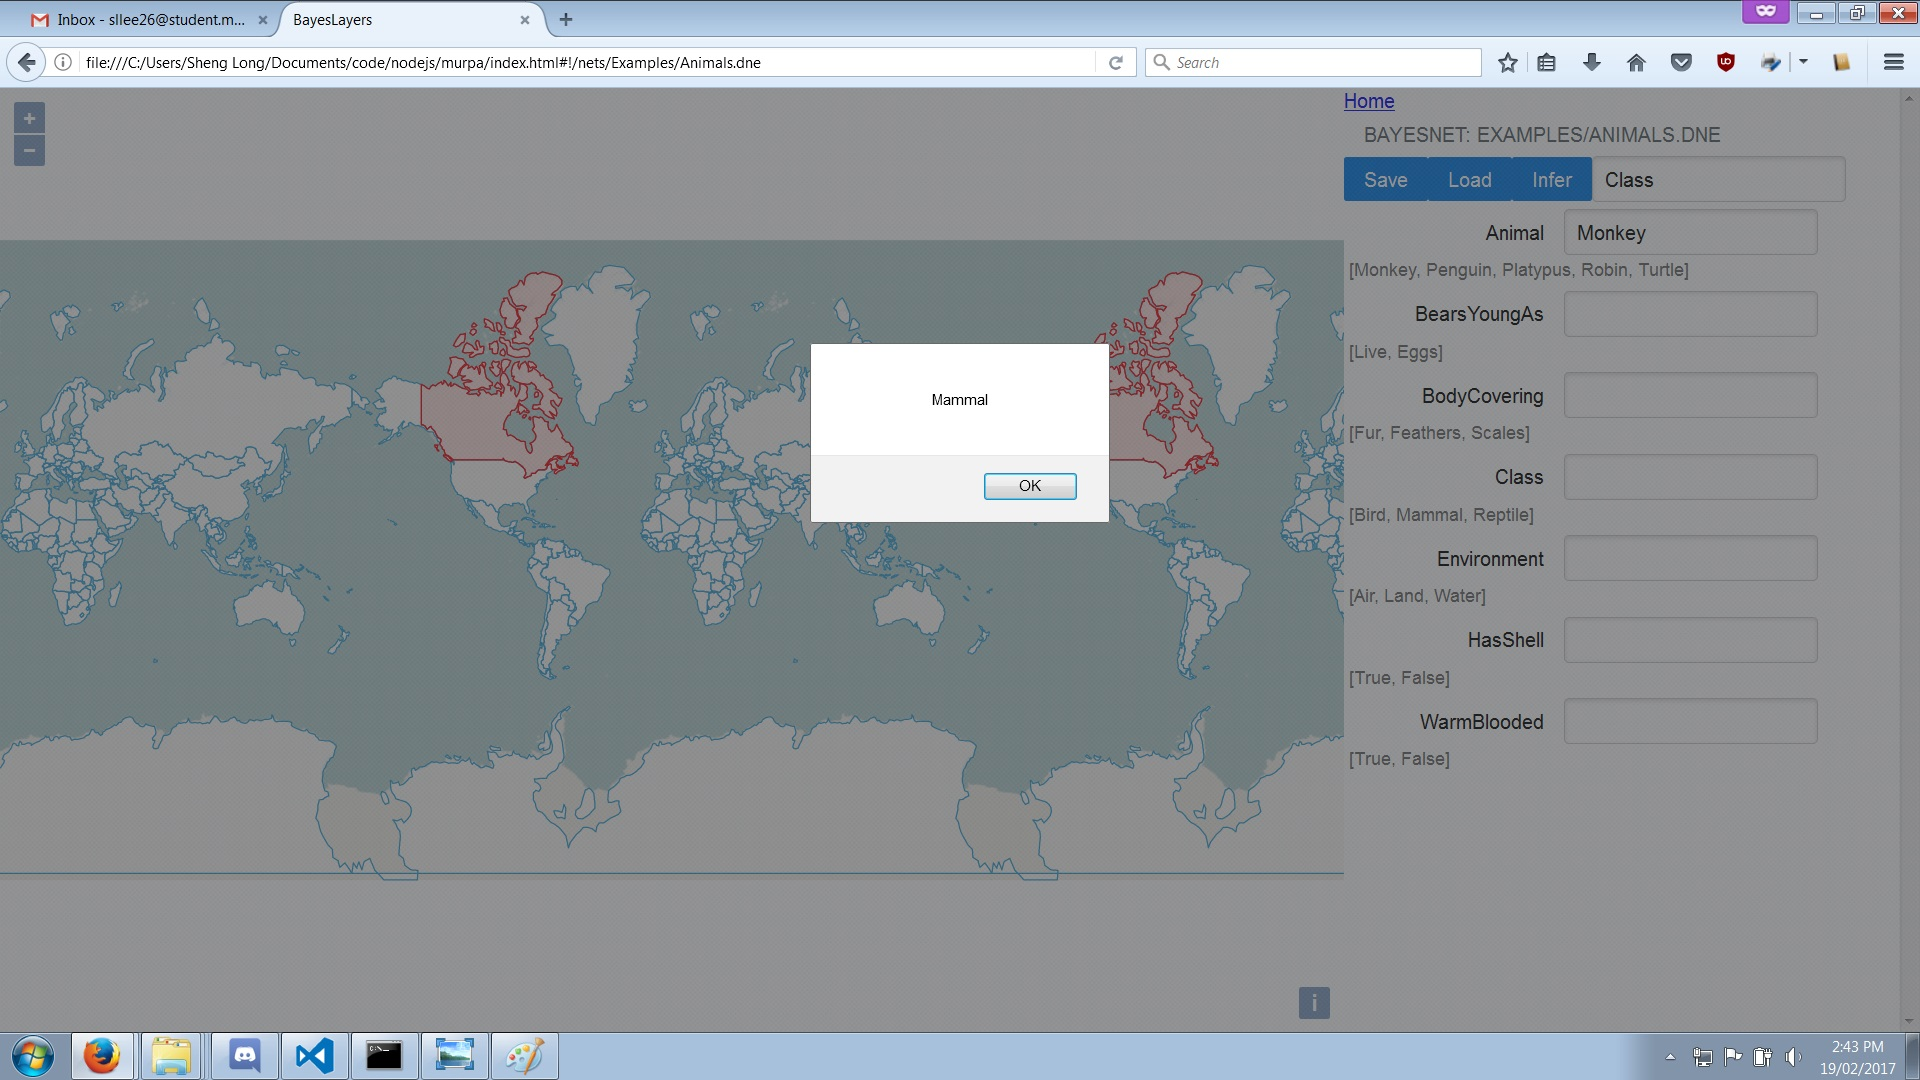
\includegraphics[width=0.8\linewidth]{v0infer}
\end{center}
\subsection{GUI screenshots after departure}\label{subsec:screens1}
The text inputs have been replaced with dropdown menus where it made sense.
\begin{center}
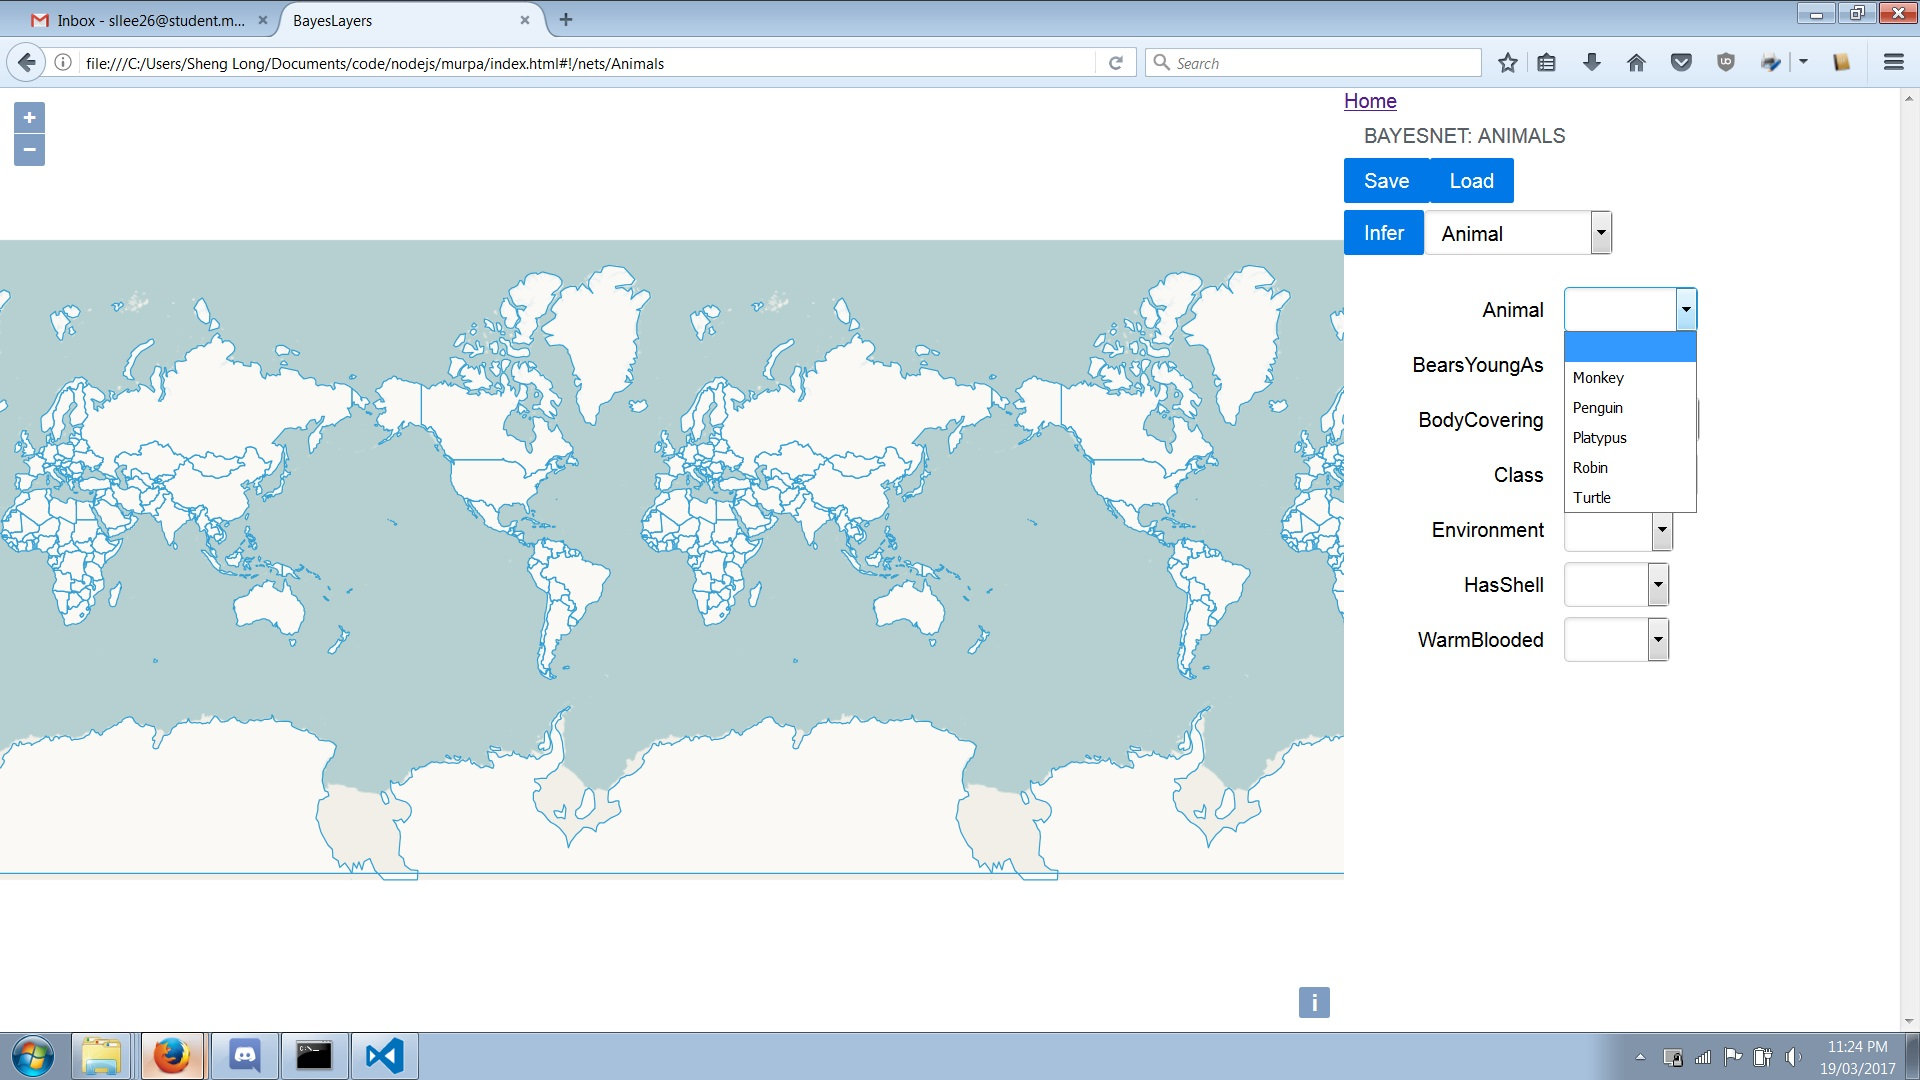
\includegraphics[width=0.8\linewidth]{v1nodes}
\end{center}
\end{document}